% Name: Circumcircle of a triangle
% Description: The perpendicular bisectors of the three sides meet at the circumcenter O, the center of the circle through A, B, and C.
% Tags: circumcircle, circumcenter, perpendicular bisector, triangle centers

\usetikzlibrary{calc, angles}

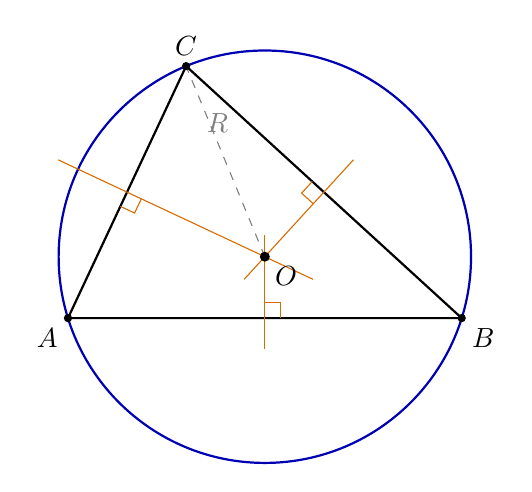
\begin{tikzpicture}[thick]
  % For A(0,0), B(5,0), C(1.5,3.2): O = (2.5, 0.7797) and R = OA = 2.6188
  \coordinate[label=below left:$A$] (A) at (0,0);
  \coordinate[label=below right:$B$] (B) at (5,0);
  \coordinate[label=above:$C$] (C) at (1.5,3.2);
  \coordinate (O) at (2.5,0.7797);
  \draw[blue!70!black] (O) circle (2.6188);
  \draw (A) -- (B) -- (C) -- cycle;
  \foreach \p/\q in {A/B, B/C, C/A} {
    \coordinate (M) at ($(\p)!0.5!(\q)$);
    \draw[orange!85!black, thin] ($(M)!-0.5!(O)$) -- ($(M)!1.35!(O)$);
    \pic[draw=orange!85!black, thin, angle radius=2mm] {right angle=\q--M--O};
  }
  \draw[gray, dashed, thin] (O) -- node[above, pos=0.6] {$R$} (C);
  \fill (O) circle (1.8pt) node[below right] {$O$};
  \foreach \p in {A, B, C} \fill (\p) circle (1.5pt);
\end{tikzpicture}
